\documentclass[11pt,oneside,a4paper]{article}
%define the title
\usepackage{graphicx}
\usepackage{listings}
\usepackage{setspace}
\usepackage{float}
\usepackage{titlesec}
\usepackage{amssymb}
%\usepackage{indent}
%\usepackage[labelfont=bf, textfont=normalfont, singlelinecheck=off, justification=raggedright]{caption}
% \titleformat*{\section}{\Large}
% \titleformat*{\subsection}{large}
% \titleformat*{\subsubsection}{normalsize}
\author{Group}
\title{Final_Report}
\begin{document}
\begin{titlepage}
\begin{center}
{\large \textsc{COMP2043.GRP Interim Group Report}}

\vspace{0.025\textheight} % Whitespace between the title and short horizonta
{\huge \textsc{Sequential Monte Carlo}} % Author name

\vspace{0.045\textheight}
{\huge\textsc{Team 6}}
\vspace{0.05\textheight}

{\huge\textsc{ 2017.12.7}}
\vspace{0.45\textheight}


\textbf{Supervisor:} Dr. Liang Dai
\vspace{0.045\textheight}

\textbf{Member:}
\begin{spacing}{2.0}%%�м�����Ϊdouble-space
          Hejia Qiu zy18720

          Cong Liu zy19426

          Zexi Song zy15777

          Xiang Zhang zy18743

          Kaiwen Zhang zy18672
\end{spacing}
  	\vspace{0.025\textheight}
\end{center}
\end{titlepage}
\tableofcontents
\newpage
\section{Introduction}

\subsection{Background of the Project}
Sequential Monte Carlo(SMC, also called particle filter), is a widely-used statistical sampling method, which is
used to sequentially sample from a sequence of target densities. It deals with the problem of recursively estimating
the probability density function $ p(x_t|Y_s) $.
\newline Befort the short journey of Introduction to Particle filter, a brief Background of particle filter will be explained in advanced. In our present world, the ability
of solve the problem of estimating various quantities in nonlinear dynamic systems is of paramount importance in many
practical applications. In order to understand how a system, for instance, a aircraft, a car, or a camera performs, we
need to have access to certain important quantities related with the system. However, typically we have to estimate them
based on various noisy measuremets available from the sytem due to the fact that we do not have direct access to these factors.
According to Thomas B.Schon, the state estimation problem is addressed mianly within a probabilistic framework. More specifically,
the approach is heavily affected by the Bayesian view of estimation, which implies that the complete solution to the
estimation problem is provided by the probability density function $ p(x_t|Y_s) $. This density function contains all available
information about the state variable.

\subsection{Motivation \& Wide implmentation of state estimation}
This section illustrates the kind of problems that can be handled using state estimation, by explaining two applications. For instance, first of all, the automotive industry's focus is recently shifting from mechanics to electronics and software. This opens up factors
a great deal of interesting applications and research opportunities within the field of estimation theory.
\begin{figure}[H]
  \begin{center}
  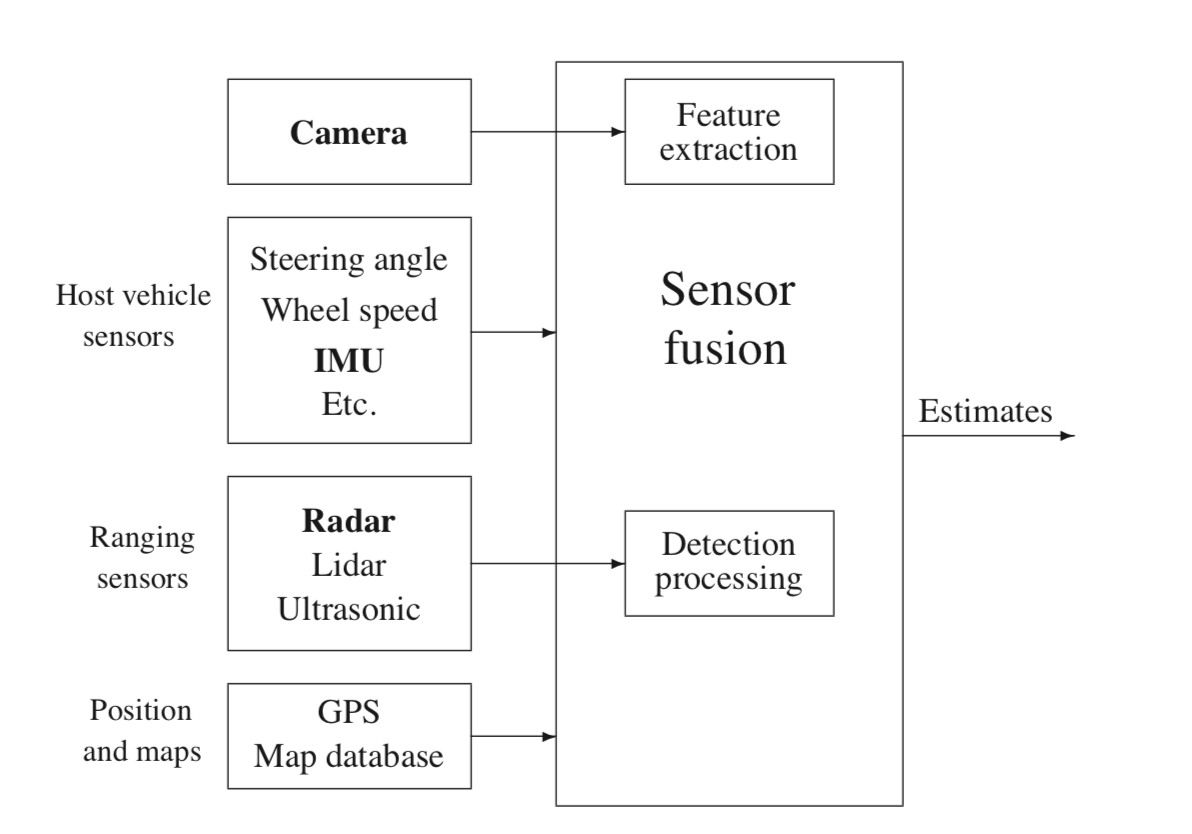
\includegraphics[height=0.3\textheight]{./source/PF/1.png}
  \end{center}
  \caption{ The most important factors enabling future automative safety systems
  is the availablility of accurate information about the state. The process of obtaining
  this information is to a large extent dependent on a unified treament of the sensor information, as illustrated
  in this figure.}
  \label{}
\end{figure}
\subsubsection{Automotive Navigation-Example}
The objective of this study is to calculate estimates of the road geometry,
which are important in several advanced control systems such as lane guidance
and collision avoidance. The idea exemplified here follows from the general framework introduced in Figure 1.

\begin{figure}[H]
  \begin{center}
  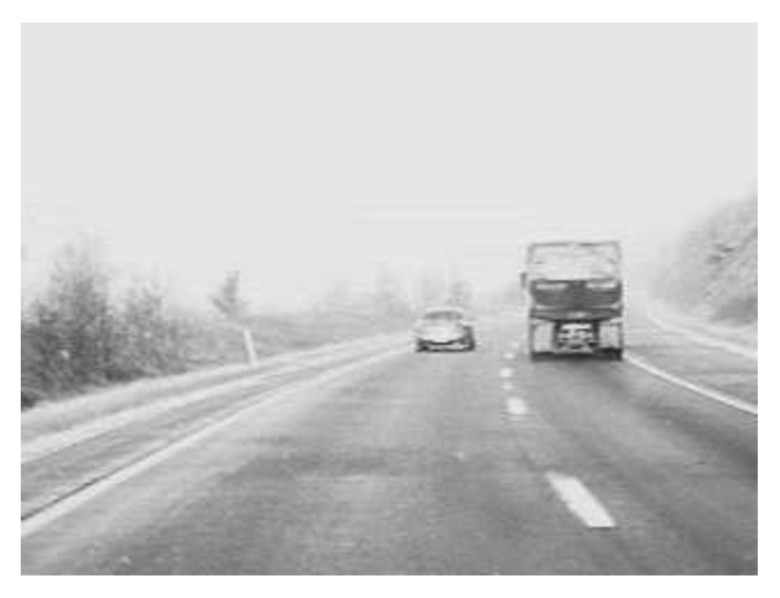
\includegraphics[height=0.3\textheight]{./source/PF/2.png}
  \caption{when entering a curve, all vehicles start moving in the lateral direction. This information
  can be used to support the road geometry estimate.}
  \label{}
  \end{center}
\end{figure}
Here information from several sensors is used to obtain better perfomance, than separate use of the sensors would allow for.The main
assumption is that the leading vehicles will keep following their lane, and their lateral movement can thus be used to support the otherwise
difficult process of road geomtry estimation. For instance, when entering a curve as in Figure 2 the vehicles ahead will start moving to
the right and thus there is a high probability that the road is turning to the right.
Assuming that the surrounding vehicles will keep following the same lane, is in discrete-time expressed as
$y{_t+1}^i = y_{t}^i + w_t,\qquad w_t \sim \mathcal{N}(0, \mathcal{Q}_{lat}). $ Here, $y^i $ denotes the lateral
position of vehicle $i $ and $w_t $ denotes Gaussian white noise which is used to accout for model uncertainties.
The estimate of the road curvature during an exit phase of a curve is illustrated in Figure 3. The true reference
signal was generated using the method proposed by Eidehall and Gustafsson (2006).

\begin{figure}[H]
  \begin{center}
  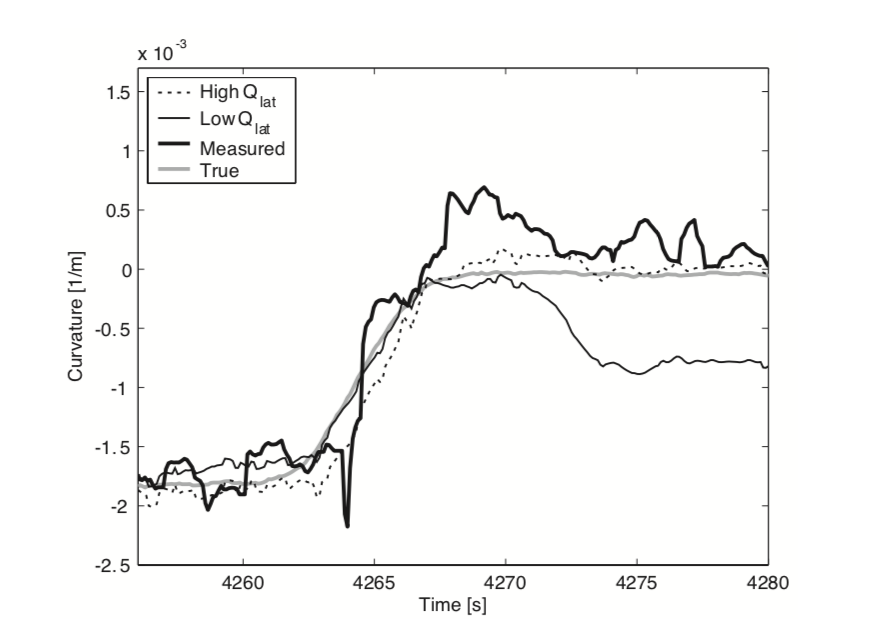
\includegraphics[height=0.3\textheight]{./source/PF/3.png}
  \caption{Comparision of estimation performance from two filters, one with a large $\mathcal{Q}_{lat} $ and one with a small $\mathcal{Q}_{lat} $. The raw measuremet signal from the image processing
  unit is also included. Comparing this raw vision measuremet to the result from the filters clearly illustrates the power of a model based sensor fusion approach}
  \label{}
  \end{center}
\end{figure}

\subsubsection{Navigation for Augmented Reality}
\begin{figure}[H]
  \begin{center}
  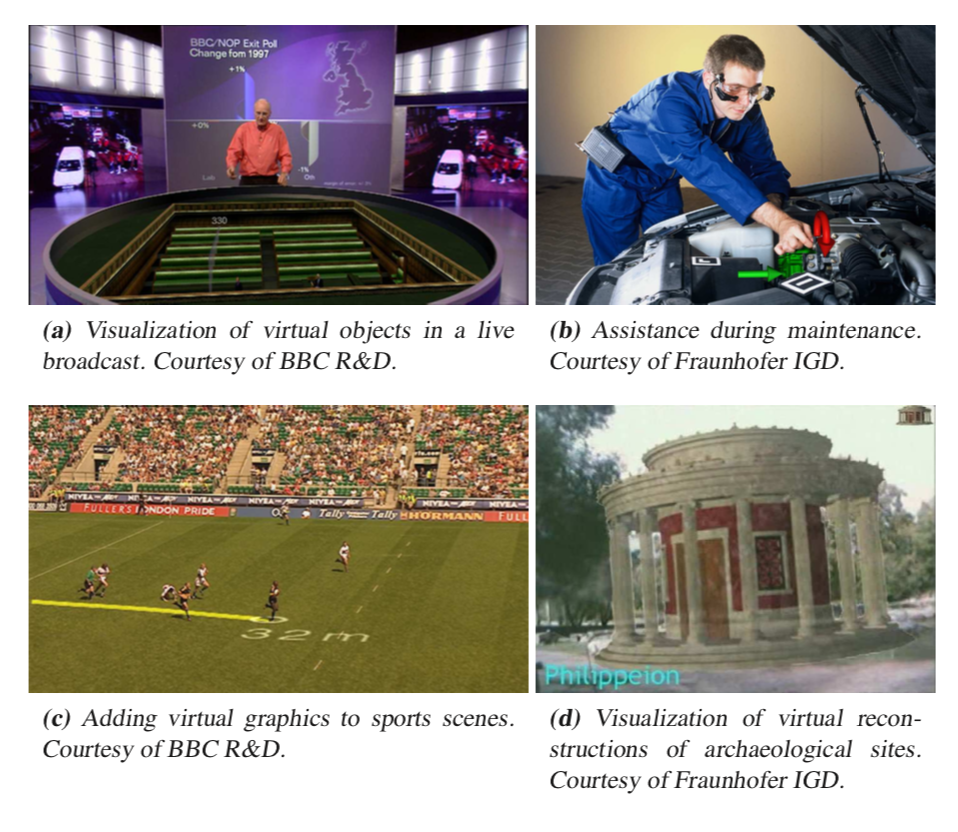
\includegraphics[height=0.35\textheight]{./source/PF/4.png}
  \caption{Some examples illustrating the concept of augmented reality.}
  \label{}
  \end{center}
\end{figure}

\subsection{Scope of the project}
This subsection describes the scenario where the product will be used for.

\subsection{Introducing two kinds of auxiliary particle filters(APF)}
\subsubsection{Sequential Monte Carlo Methods}
As we have mentioned above that Sequential Monte Carlo methods, or particle methods, provide the solution for state estimation. Then, what does it
constitue? It is constituted by a combination of sequential importance sampling and resampling. The key idea underlying the particle methods is to represent
the probability density function by a set of samples(also referred to as particles, hence the name particle methods) and its associated weights.
The density function $p(x_{t}|Y_s) $ is approximated with an empirial density function,
\begin{equation}
p(x_{t}|Y_s) \approx \sum_{i=1}^M\tilde{q}_t^{(i)}\delta(x_t - x_{t|s}^{(i)}), \qquad \sum_{i=1}^{M}\tilde{q}_{t}^{(i)} = 1, \qquad \tilde{q}_{t}^{(i)} \geq 0, \forall{i}
\end{equation}
where $\delta(\cdot) $ represents the Dirac delta function and $\tilde{q}_{t}^{(i)} $ denotes the weight associated with particle $x_{t|s}^{(i)} $. For intuition we can think of each
particle $x_{t}^{i} $ as a possible system state and the corresponding weight $\tilde{q}_{t}^{(i)} $ contains information about how probable that particular state is.
\begin{figure}[H]
  \begin{center}
  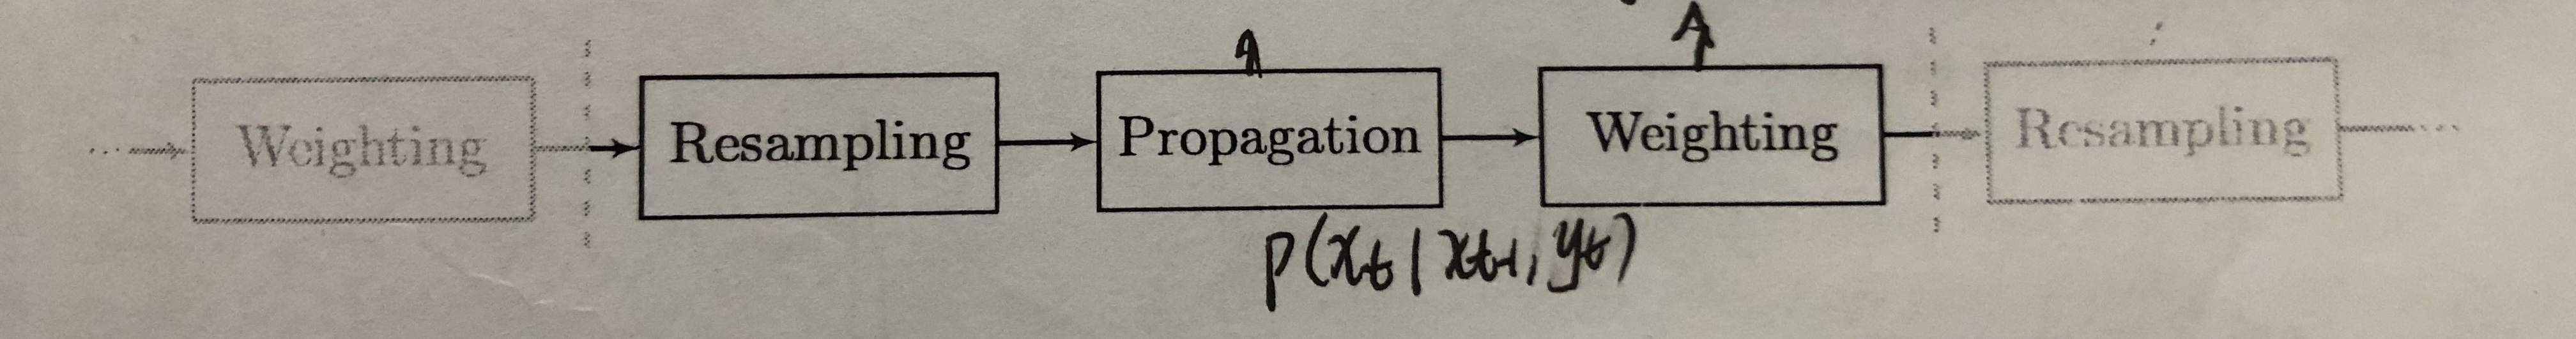
\includegraphics[width=0.9\textwidth]{./source/PF/5.JPG}
  \caption{Illustrating the three parts making up sequential Monte Carlo}
  \label{}
  \end{center}
\end{figure}

\subsubsection{Auxiliary particle filter(APF)}
As a principled solution to compute the filtering PDFs $ \lbrace (x_{t}|y_{1:t}) \rbrace $ sequentially in time is provided by the following
two recursively equations:
\begin{equation}
p(x_{t} | y_{1:t}) = p(x_t | y_t, y_{1:t-1}) = \frac{p(y_t|x_t)p(x_t|y_{1:t-1})}{p(y_t|y_{1:t-1})}
\end{equation}
\begin{equation}
p(x_{t} | y_{1:t-1}) = \int p(x_t|x_{t-1})p(x_{t-1}|y_{1:t-1}) d_{x_{t-1}}
\end{equation}
These two equations are coming from Forward filtering. The explaination will be included in the Appendixes in detail. Further, the main barrier here is the integral in equation (3), which is in general
not analytically tractable. Nevertheless, the integral can be approximated using an importance sampler targeting the filtering distribution at time $ t-1 $. This give us the impetus to proceed in an inductive
fashion. Thus,assuming we have an empirial approximation of the filtering distribution at time t-1, constituted by N weighted samples, $\{ x_{t-1}^i, w_{t-1}^i \}_{i=1}^{N} $, i.e.
\begin{equation}
\hat{p}^N(x_{t-1}|y_{1:t-1}) = \sum_{i=1}^N w_{t-1}^i\delta_{x_{t-1}^i}(x_{t-1})
\end{equation}
At time $t = 1 $, it is able to obtain a point-mass approximation according to eqution (4), by targeting $p(x_{1}|y_{1}) \propto p(y_{1}|x_{1})\mu{(x_{1})} $ with an importance sampler. Inserting the approximation
$\hat{p}^N(x_{t-1}|y_{1:t-1}) $ into equaiton(3), result in
\begin{equation}
\hat{p}^N(x_{t}|y_{1:t-1}) = \int p(x_{t}|x_{t-1}) \sum_{i=1}^{N} w_{t-1}^{i}\delta_{x_{t-1}^{i}}(x_{t-1})d_{x_{t-1}} = \sum_{i=1}^{N}w_{t-1}^{i}p(x_{t}|x_{t-1}^{i})
\end{equation}
Using equation(5) and equation(2), we can evaluate an approximation of the filtering PDF $p(x_t|y_{1:t} $ up to proportionality
\begin{equation}
p(x_{t}|y_{1:t}) \approx \frac{1}{p(y_t|y_{1:t-1})} \sum_{i=1}^N w_{t-1}^i p(y_t|x_t)p(x_t|x_{t-1}^i)
\end{equation}
As for this opens up for targeting $p(x_{t}|y_{1:t}) $ with an importance sampler. Then, choosing a similar type of mixture
as proposal density, namely
\begin{equation}
q(x_{t}|y_{1:t}) = \sum_{i=1}^N w_{t-1}^i q(x_t|x_{t-1}^i,y_t)
\end{equation}
There are many different options when it comes to choosing the component $q(x_{t}|x_{t-1}^{i}, y_{t}) $ in this mixture. Note that, in general, the proposal density at time $t $ is allowed to depend on the current
observation $y_{t} $, as indicated by the notation used in equation (7). Therefore, Using auxiliary variable in the form of a discrete random variable $a_{t} $ which takes values on the set of integers $\{ 1,...,N\} $ in the $q(x_t|y_{1:t}) $ can take $y_{t} $ into account, which make use of this information already when simulating
the particles $\{ x_{t}^{i} \}_{i=1}^{N} $, to increase the probability of producing samples in the most relevant parts of the state space. This is why we indicate a possible dependence on $y_{t} $ in the mixture components of
the proposal density in (7).The key in this development is to target the joint distribution of $(x_{t}, a_{t}) $ with an importance sampler, instead of directly targeting the marginal
distribution of $x_{t} $\\
Analogously to above, the mixture proposal (7) can be interpreted as a joint proposal distribution for the pair $(x_{t}, a_{t}) $, given by
\begin{equation}
q(x_{t}, a_{t} | y_{1:t}) = w_{t-1}^{a_t}q(x_{t}|x_{t-1}^{a_{t}}, y_{t})
\end{equation}
Here, $a_{t} $ should be thought of as an index selecting one of the componets in the sum (7).
Generating, independently, N realizations from this joint proposal distribution can be done as follows.
\flushleft
\begin{enumerate}
\item Sample the ancestor indices $ \{ a_{t}^{i} \}_{i=1}^{N} $ according to
\begin{equation}
\mathbb{P} (A_{t} = i \arrowvert \{ x_{t-1}^{j}, w_{t-1}^{j} \}_{j=1}^{N} ) = w_{t-1}^{i} \qquad i = 1,...,N
\end{equation}
This corresponds to the resampling step of the algorithm. The resampled particles are given as $ \bar{x}_{t-1}^{i} = x_{t-1}^{a_{t}^{i}} $ for $ i = 1,...,N $.
\item Propagate the particles to time t by simulating $x_{t}^{i} \backsim q(x_{t}| \bar{x}_{t-1}^{i}, y_{t}) $ for $i = 1,...,N $
\end{enumerate}
The advantage of explicitly introducing and implmenting auxiliary variable lies in the computation of the importance weight. From (6),
we have that the joint target distribution for $(x_{t}, a_{t}) $ is proportional to what called unnormalized joint target density:
\begin{equation}
w_{t-1}^{a_{t}}p(y_{t}|x_{t})p(x_{t}|x_{t-1}^{a_{t}})
\end{equation}
In fact, it is possible to use the information available in the current observation $y_{t} $, not only when proposing the new state $x_{t} $, but also when proposing its ancestor index $a_{t} $. The principle is that we can thereby increase the probability of resampling particles at time $t-1 $ that are in
agreement with the observation $y_{t} $. \\
It is free to use any proposal distribution that we find appropriate to obtain the pair $(x_{t}, a_{t}) $ (Thomas B. Schon, Fredrik Lindsten, 2017). For example, let $v $ be the function that will be used to adapt the proposal distribution for the ancestor indices. For each particle
, i.e. for $i = 1,...,N $, we then compute the quantities
\begin{equation}
  v_{t-1}^{i} := v(x_{t-1}^{i}, y_{t}),
\end{equation}
referred to as adjustment multipliers. The adjustment multipliers are used to construct a proposal distribution for the ancestor index variable $a_{t} $
\begin{equation}
\mathbb{P} (A_{t} = i \arrowvert \{ x_{t-1}^{j}, w_{t-1}^{j} \}_{j=1}^{N} , y_{t} ) = \frac{w_{t-1}^{i} V_{t-1}^{i}}{\sum_{t=1}^{N} w_{t-1}^{l} v_{t-1}^{l}} \qquad i = 1,...,N
\end{equation}
From the above expression, it is clear that v acts as adjusting the original weights $w $ via multiplication. The underlying ideas of implementation of adjustment multipliers is that by carefully choosing the function $v $, we can adapt the sampling of the ancestor
indices in equation (12) to make use of the information available in the current measuremet $y_{t} $ \\
Then, we get the following expression for the $i $ importance weight as the use of adjustment multipliers:
\begin{equation}
\bar{w}_{t}^{i} = w(x_{t-1}, x_{t}, y_{t}) = \frac{w_{t-1}^{a_{t}^{i}} p(y_{t}|x_{t}^{i}) p(x_{t}^{i}|x_{t-1}^{a_{t}^{i}})}{w_{t-1}^{a_{t}^{i}} v(\bar{x}_{t-1}, y_{t}) q(x_{t}^{i}|x_{t-1}^{a_{t}^{i}}, y_{t})}
\end{equation}
This completes the algorithm, since these weighted particles in turn can be used to approximate the filtering PDF at
time t+1, then at time t+2 and so on.


\subsubsection{Bootstrap particle filter}
After we have known the Auxiliary particle filter, a pragmatic solution for bootstrap particle filter is to choose the proposal density according to
\begin{equation}
w_{t-1}^{a_{t}^{i}} v_{t-1}^{a_{t}} = w_{t-1}^{a_{t}},
\end{equation}
\begin{equation}
q(x_{t}|x_{t-1}^{a_{t}}, y_{t}) = p(x_{t}|x_{t-1}^{j}),
\end{equation}
\begin{equation}
q(x_{t}, a_{t} | y_{1:t}) = \sum_{j=1}^{N}w_{t-1}^{j}p(x_{t}|x_{t-1}^{j})
\end{equation} \\
Therefore, it follows that the weight function is given by
\begin{equation}
\bar{w}_{t}^{i} = \frac{w_{t-1}^{a_{t}^{i}} p(y_{t}|x_{t}^{i}) p(x_{t}^{i}|x_{t-1}^{a_{t}^{i}})}{w_{t-1}^{j}p(x_{t}|x_{t-1}^{j})} = p(y_{t}|x_{t})
\end{equation}
This completes the algorithm.
\begin{figure}[H]
  \begin{center}
  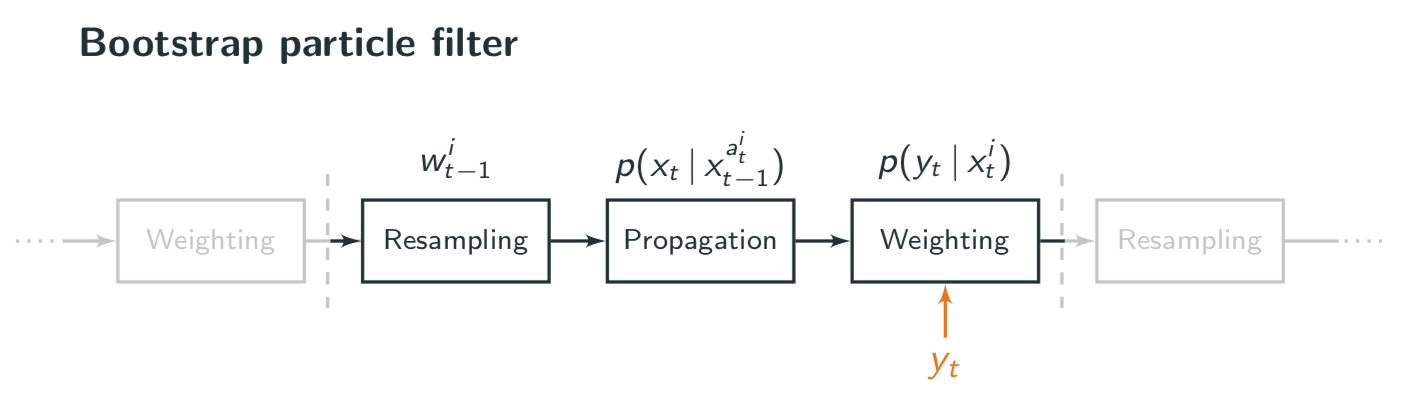
\includegraphics[width=0.9\textwidth]{./source/PF/6.png}
  \caption{bootstrap particle filter}
  \end{center}
  \label{}
\end{figure}
\subsubsection{Fully adapted particle filter}
In order to adapt the proposals to the information that is available in the current observation $y_{t} $. A nature choice as for the proposal for the state $x_{t} $ is to use
\begin{equation}
  q(x_{t}|x_{t-1}, y_{t}) = p(x_{t}|x_{t-1}, y_{t}),
\end{equation}
From Bayes'rule, we can write
\begin{equation}
  p(x_{t}|x_{t-1}, y_{t}) = \frac{p(y_{t}|x_{t}) p(x_{t}|x_{t-1})}{p(y_{t}|x_{t-1})},
\end{equation}
Plugging this expression into the denominator of equation (13) we obtain
\begin{equation}
\bar{w}_{t}^{i} = w(x_{t-1}, x_{t}, y_{t}) = \frac{p(y_{t} | x_{t-1})}{v(x_{t-1}, y_{t})},
\end{equation}
When it confront the choice to decide the adjustment multipliers. In particular, we see the choice $v(x_{t-1}, y_{t}) = p(y_{t}|x_{t-1}) $ will lead to a weight function that is identically equal to 1. In other word, we obtain particles that are generated in such a way that they are equally informative about the
target distribution.
\begin{equation}
  \bar{w}_{t}^{i} = 1.
\end{equation}
This completes the algorithm.
\begin{figure}[H]
  \begin{center}
  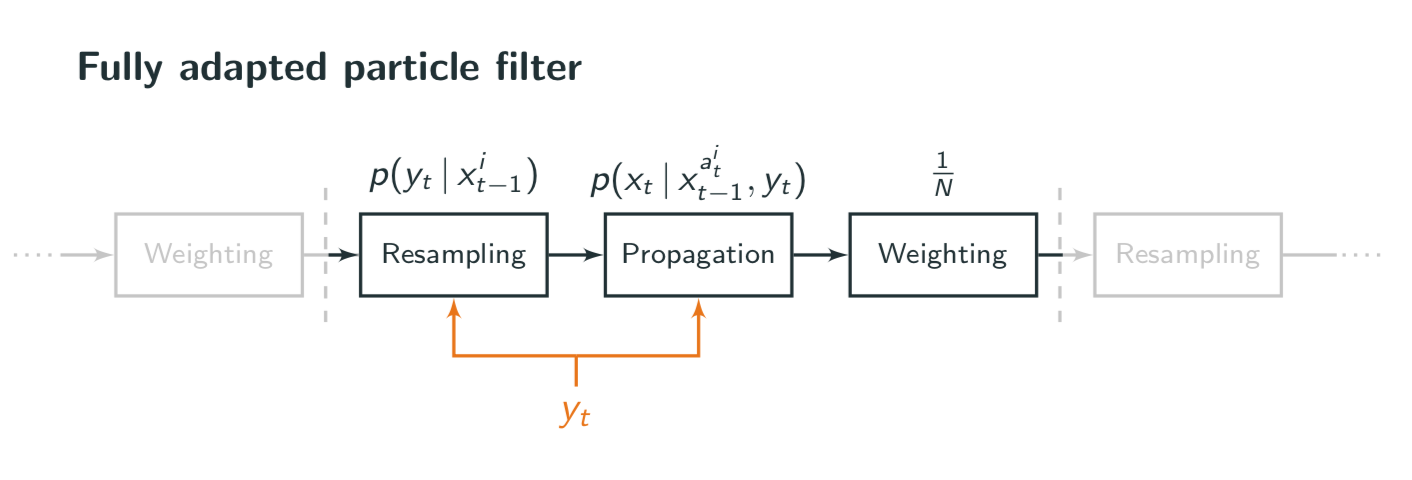
\includegraphics[width=0.9\textwidth]{./source/PF/7.png}
  \caption{Fully adapted particle filter}
  \label{}
  \end{center}
\end{figure}

\section{Requirement Specification}
\subsection{Introduction}
Particle Filter Simulator is a lightweight application which is mainly used by college students and teachers. Because Particle Filter Simulator is aimed for teaching or image and data processing, thus, in order to meet the main needs of users and provide positive user experience,
a large amount of significant requirements should be carefully considered and implemented. In this part of report, it will illustrate the process of gathering and implementing requirement and provide a list of different types of requirements. For each specific requirement,
it will be analyzed and explained in more details.
\subsection{User case Diagram}
Use case diagram could describe how users interact with system and it could be the first step from requirement specification to software implementation. The actors, use cases and system boundary will be shown as follow. It could help developers implement the main function of Particle Filter Simulator and provide a clear diagram for users to understand each parts of the software.
\begin{figure}[H]
  \begin{center}
  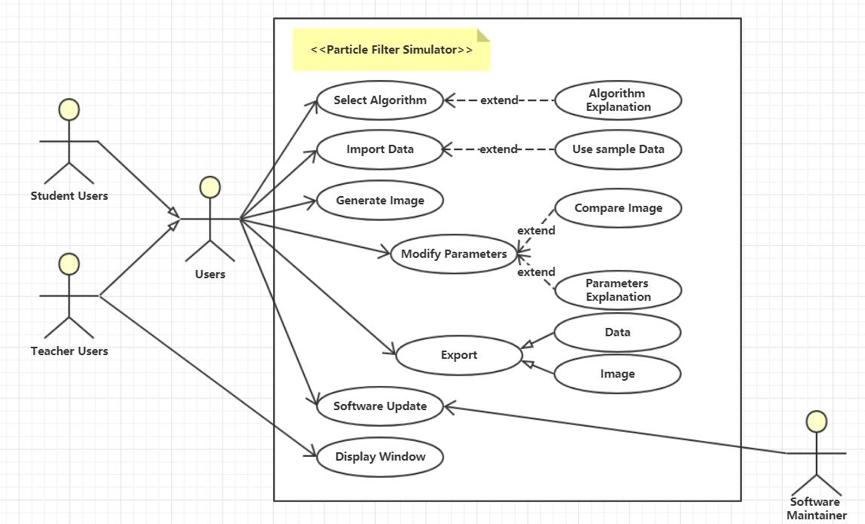
\includegraphics[height=0.4\textheight]{./source/Requirement/1.png}
  \caption{User case diagram}
  \label{}
  \end{center}
\end{figure}

\subsection{Prototype}
Software prototype provides a brief user interface and it has been divided the whole software into several parts. Developer could better implement division and cooperation by focusing on each different component in prototype. It also provides a feasible option to validate if the software design achieves expected user experience.
\begin{enumerate}
  \item Start interface: After the software is opened by user, user should first select different algorithms. It is the first impression of user experience and help users gets start easily.
  \begin{figure}[H]
    \begin{center}
    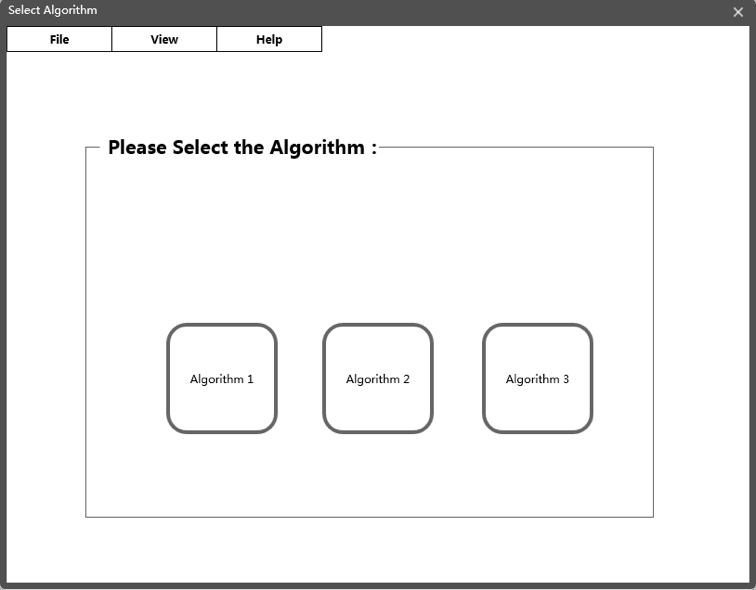
\includegraphics[height=0.3\textheight]{./source/Requirement/2.png}
    \caption{Start interface}
    \label{}
    \end{center}
  \end{figure}

  \item Navigating bar: Navigating bar is placed on the top of window and it contains three main options: File, View and Help. File options include the function of operating input and output file. View options include the function of setting window on the top or changing the software appearance. Help options include the help document and software update.
  \begin{figure}[H]
    \begin{center}
    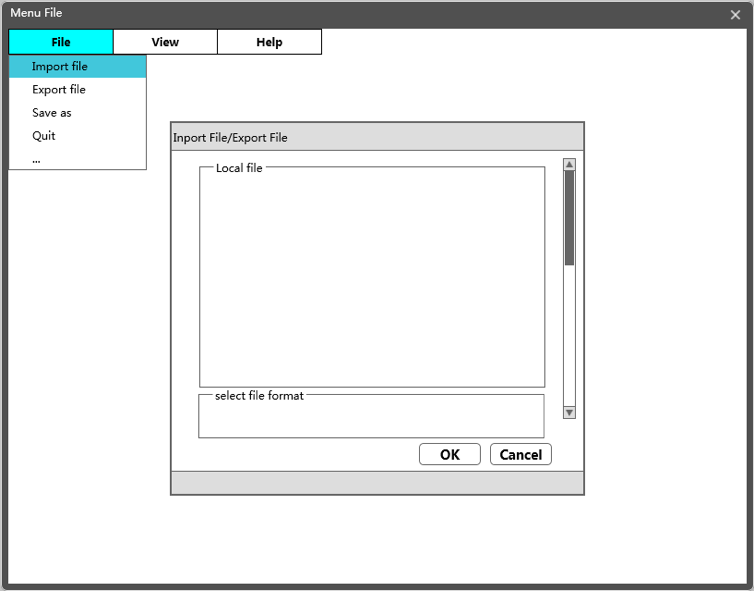
\includegraphics[height=0.3\textheight]{./source/Requirement/3.png}
    \caption{Navigating bar-File}
    \label{}
    \end{center}
  \end{figure}

  \begin{figure}[H]
    \begin{center}
    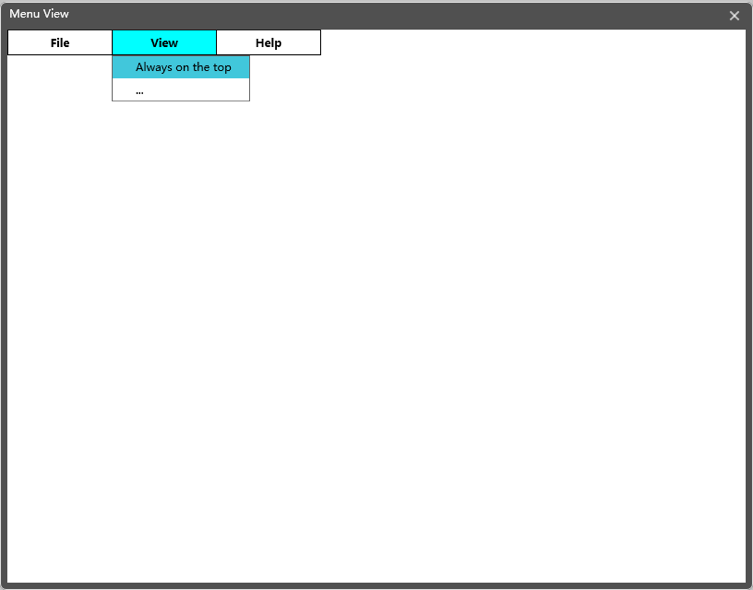
\includegraphics[height=0.3\textheight]{./source/Requirement/4.png}
    \caption{Navigating bar-View}
    \label{}
    \end{center}
  \end{figure}

  \begin{figure}[H]
    \begin{center}
    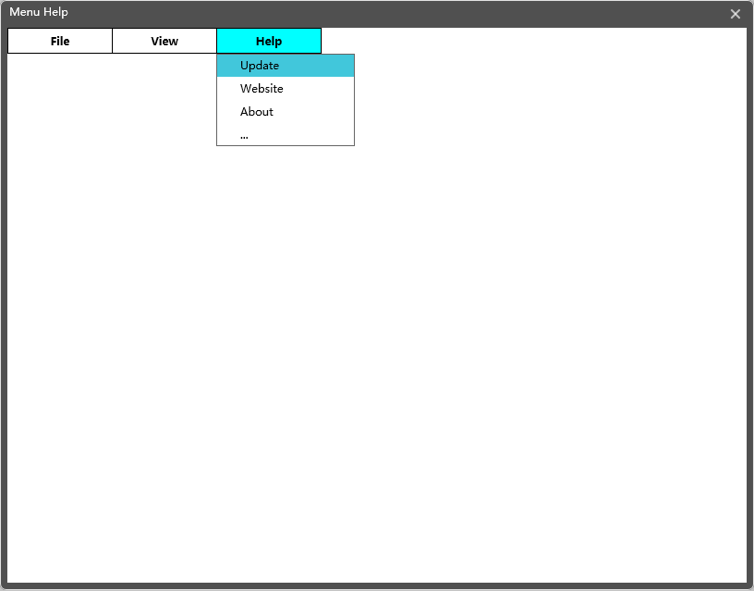
\includegraphics[height=0.3\textheight]{./source/Requirement/5.png}
    \caption{Navigating bar-Help}
    \label{}
    \end{center}
  \end{figure}

  \item Main interface: Main interface of generating data and image, which includes three components: function button, outcome image and parameter controller. Function button includes several functional buttons to deal with data and image. Outcome image includes an area to generate a plot image with coordinate axis and two scroll bar. Parameter controller contains a list containing parameter name, several slider used to adjust parameter value and a start and refresh button.
  \begin{figure}[H]
    \begin{center}
    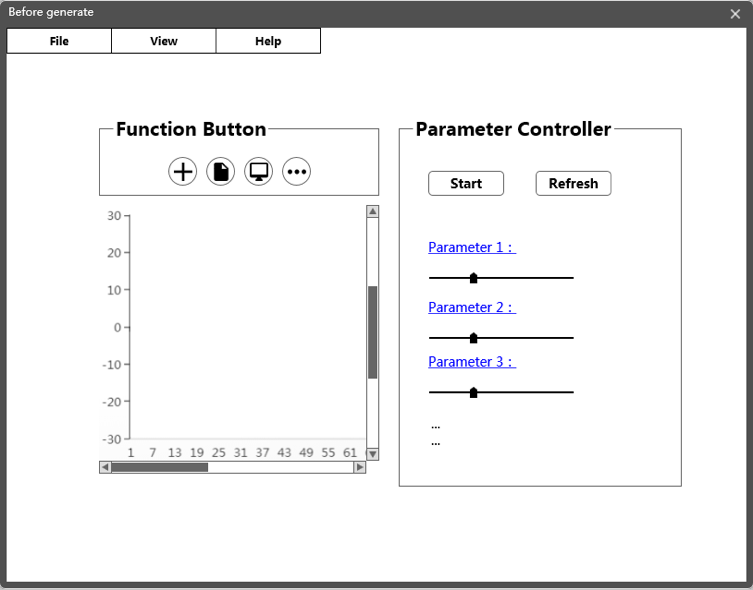
\includegraphics[height=0.3\textheight]{./source/Requirement/6.png}
    \caption{Main interface-prepare}
    \label{}
    \end{center}
  \end{figure}

  \begin{figure}[H]
    \begin{center}
    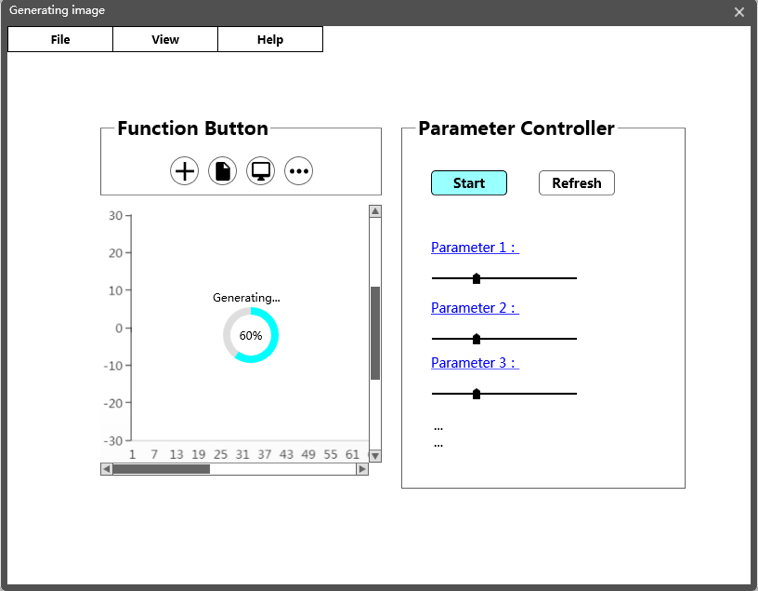
\includegraphics[height=0.3\textheight]{./source/Requirement/7.png}
    \caption{Main interface-executing}
    \label{}
    \end{center}
  \end{figure}

  \begin{figure}[H]
    \begin{center}
    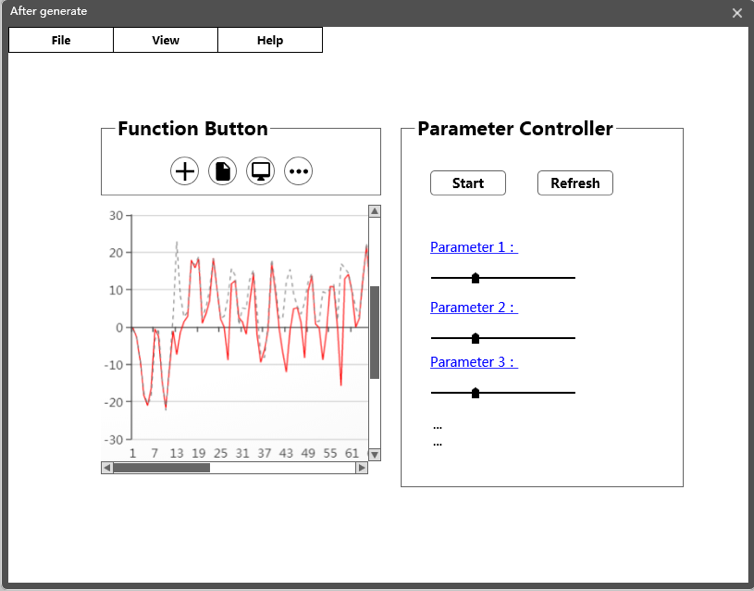
\includegraphics[height=0.3\textheight]{./source/Requirement/8.png}
    \caption{Main interface-complete}
    \label{}
    \end{center}
  \end{figure}
\end{enumerate}
\subsection{Requirements list}
During the procedure of software design and requirements Implementation, developers found that some requirements is difficult to implement and there are also some new requirements need to be considered. In this section, it mainly focusing on the requirements that has been appeared in the software design process and which of them have been implemented or not.
\subsubsection{Functional requirements}
Particle Filter Simulator is using the algorithm selected by user to generate the outcome image. These are the main functional requirements appearing during the software design process:
\begin{enumerate}
  \item The software should illustrate the correctly usage method in help document.
  \item The software should provide the function of selecting different algorithms
  \item The software should display the brief explanation of algorithms when user is selecting an algorithm.
  \item The software should provide some existing sample data to users without other specific data.
  \item The software needs prompt and check the format of the file when users import specific sample data.
  \item The software should use the algorithm which is selected by user to deal with the import sample data and generate the outcome image.
  \item The software should provide modifiable parameter list and brief explanations of each parameter.
  \item The software should have the function of modifying parameters which are initially set as default value.
  \item The software should implement the function of exporting images, data, or both of them according to the user’s decision.
  \item The software should permit users to combine two images together to compare the differences between them.
  \item The software should provide the function of clearing the current data and results if users want to import another sample data or select another algorithm.
  \item The software should provide a function of putting the software window into the top.
  \item A restart button should be provided to handle the situation of software crashing.
  \item The software need to check version update automatically and submit bugs which are collected by users to software maintainer.
  \item When the software is using algorithm to generate image, a progress bar or a waiting hint should be provided which is used to display the running state of software.
  \item The range of permanents should be limited to avoid the situation that increasing running time of algorithm and software crashing.
\end{enumerate}

\subsubsection{Non-functional requirements}
Performance \& security \& Environment:
The non-functional requirements are given as follow which include the environment requirements, performance requirements and data requirements:
\begin{enumerate}
  \item The window size of the software should be suitable for demonstration.
  \item The user interface should be convenient for user activity.
  \item The running time of using the algorithm to deal with the sample data should be as quick as possible, for instance, it should be less than 5 seconds with the consideration of the computability of Javascript.
  \item The system resources occupied by software should be limited.
  \item The software needs to run on major platforms and operating systems.
  \item The software should be convenient for update and extension.
  \item The outcome image should have positive distributing accuracy when the value of several parameters is limited.
  \item The software requires appropriate software capacity to be convenient for users download and use in a short period of time.
  \item It should be convenient to passing parameter data between each component in different part of software.
  \item The software is free, it is better that the development and maintenance costs should be properly reduced.
\end{enumerate}

\section{Development Strategies}
\subsection{Agile}
Stakeholders:
\begin{enumerate}
  \item Teachers: Teachers might use this software to help explaining particle filter for academic purpose. Main requirement of this system is visualizing the output of the algorithm. Before the visualization, teacher will be able to set the parameters of particle filter, then the algorithm will run in the background based on Bayes theorem.
  \item Student: Students require same functions as teacher and expect that this software will be providing data import/export functions. By those functions they can compare output of the algorithm with different parameters, in the form of both data and visual image. Those functions can also be used to submit the output to teacher if required.

\end{enumerate}
\subsection{Techiniques}
As this software is designed as an academic teaching tool and might run on school’s or users’ own machine, we are supposed to choose techniques that are available to develop light-weight and cross-platform PC application.
The realizability of data visualization and algorithm computation is the basic requirement of choice.
Learning cost and whether suitable for cooperative development will also be considered as the develop group is supposed to learn and develop as a team.

\subsection{Plan \& Task assignments}
\begin{enumerate}
  \item For this group project, as it is based on complex mathematical knowledge, two members mostly focus on the realization of the algorithm, including the implementation of the algorithm in background code and related documents. (Cong Liu & Kaiwen Zhang)
  \item One member is responsible for choosing developing techniques, including developing language, framework and tool components. He is also supposed to set up the software development framework and help other members building the develop environment and solve technique problems in developing. (Hejia Qiu)
  \item One member will cooperate with the former one to develop the software, both in design an d code, and supposed to complete some functions and test work. Prototype and interface design is also supposed to complete by this member with the technique chooser. (Xiang Zhang)
  \item As this group project requires meeting and documents, one member will work as documenter to record meeting minutes and necessary documents, both for developers and users. (Zexi Song)
\end{enumerate}

\section{Design & Implementation}
\subsubsection{Programming Language for Development}
JavaScript, HTML and CSS:\\
As this project requires data visualization function, front-end is a suitable choice as there exists visualizing frameworks like Echarts.js based on JavaScript and canvas in front-end development.
Front-end developing also decrease the cost of interface development and can easily improve UI by CSS tools, such as Bootstrap.
\subsubsection{Developling framework}
Electron: \\
Electron is an open-source framework to build cross-platform desktop Apps with front-end language. It is based on Node.js and npm source.
\\
Vue.js:
Vue.js is an progressive JavaScript framework. It is approachable, versatile and performant.
The key advantage is make the software into components, which is much easier for group project as group member will not get confused by reading others’ code – they just work on their on component.

\subsubsection{Developling Tools}
Vue-cli:\\
Vue-cli is a full system for rapid Vue.js development and aims to be the standard tooling baseline for the Vue ecosystem.
By using this tool, the components structure can be much clear and easy to coop-develop.
\\
Electron-Vue:\\
The aim is to remove the need of manually setting up electron apps using vue-cli.

\subsubsection{Package Tools}
Electron-builder:\\
A complete solution to package and build a ready for distribution Electron app with “auto update” support out of the box based on npm/yarn source.
By using this tool, we can easily package the software into cross platform installation package and installation-free software. The size of package will also be small. In addition, auto-update function is also supported by this tool.

\subsubsection{Data Visualization Tools}
Echarts.js:\\
ECharts.js is a powerful, interactive charting and visualization library for browser.
The API of this framework can satisfy all requirement of the software.

\subsubsection{Math Tools}
Math.js:\\
Math.js is an extensive math library for JavaScript and Node.js and is used in this project to do matrix calculation.


\section{Test}
The test of Particle Filter Simulator software aims to discover the functional and service performance-related problems through variety test approaches. According to apposite approaches, basic errors and drawbacks on functions and logic can be detected and reduced.   Ensure that software can implement its functions as expected.

In this software, the whole functions will be tested including importing json file, exporting data, drawing chart of algorithm running  result, refreshing the chart and altering the parameter value of Particle Filter algorithm. The correctness of algorithm implementation will be tested particularly. In condition, parts of non-functional features which are significant to the software will be tested as well, for instance, system compatibility, installation and uninstallation, and performance in response time.
\subsection{Pass/Fail Criteria}
For functional features, the pass criterion applies to all of them: implement correctly without any error and warning. Otherwise, it is failed.

For non-functional features, pass or fail criteria should be considered separately.
\begin{enumerate}
  \item System compatibility: The criterion of system compatibility is whether the software can implement its functions well as a cross-platform software. Two mainstream operating systems must be satisfied, Windows and Mac OS.
  \item Installation: installation pass criterion is to verify that software works properly after installation. It is failed if installation error occurs.
  \item Uninstallation: the pass criterion of uninstallation is the software can be uninstalled clearly and has no harmful effects on the system.
  \item Performance(response time): Miller(1968) indicates there are three levels of response time for users. 0.1 to 0.2s: users may think it is immediate response.1~5s: The users feel that the interaction is basically smooth. The users will notice the delay. 8s or more: Users will follow the dialog. A prompt or progress bar is required to confirm that the system is still in process. Treat the information as a reference, the pass criterion is set to most response time of operations should be under 5s. Otherwise, a progress bar should be showed to tell users the computer does work. Response time over 5s and no prompt showed will be considered as failure.

\end{enumerate}
\subsection{Approach}
The test will use black box testing to check functions with equivalence partition testing and boundary testing, while using white box testing and unit testing to check the source code. Black box testing is a method of software testing that test the functionality with no internal structure knowledge. and it can be used to every level of software testing(Gao Tsao and Wu, 2003). In contrast, white box testing need to test the internal structures in a software. Two methods can complement each other to test the software. In addition, Matlab will be applied to support mathematical principles. 

Performance will be tested by Chrome devtools to present the response time of every operation. All test cases are manually testing.

\subsection{Summary}
To sum up above test cases, there are no logic and functions error in the software. The major issue is that it is slow to deal with complex data. Due to the data from chrome-devtools, the main time is for scripting. After investigation and analysis, this kind of slow is limited by JavaScript. There is no library for complex mathematical computation, therefore, amounts of basic computation must be written in code. It leads to the slow running time.

To solve the issue, reducing the number of calculations is the main direction. In order to achieve this goal, we are try to get a more concise algorithm and find a powerful mathematical library is needed. Maybe in next update, it will have a better running time. Other approaches like changing the way of declaration or loop to reducing calling time have a role as well and we are changing them gradually.





\section{Evaluation and Reflection}
\subsection{Assessment of the product}
After two semesters\’ study and work, we finally completed our software that realizes the data visualization of Bootstrap particle filter, nevertheless, the fully adapted particle filter has not been realized. Some assessments of the product including good and bad reviews are as follow
\begin{enumerate}
  \item The software of our group has completed most of the requirements.
  \item The size of our software packages is very small, and it is easy for customers to download and use.
  \item Our software can be cross-platform.
  \item Our software has more than one installation approaches for customers to choose. They could download an installation package or portable version to start using our program.
  \item Our software implements data visualization, the result of each change in data is straightforward on the graphics.
  \item Our software can import and export data. We can not only use an existing data to complete data visualization, but also export data according to the image that we have generated.
  \item The speed of the software is not optimized well. The software would run for 1.6 seconds if we set the number of particles to 100. But if the number is increased to 500, it would run for 7.9 seconds.
  \item Our software’s language choice is not the optimal choice, we had tried some other languages such as python. Using python could optimize operation time but it adds new problems which increase user load. For the sake of the user, we use JavaScript as the language of our software.
  \item λ	Our software has not been tested by Alpha text, also named informal acceptance test
\end{enumerate}
\subsubsection{Further improvement}
\begin{enumerate}
  \item We still have a lot of room for improvement in language selection. After lots of steps’ screening, we chose JavaScript. We do not think it is the optimal solution, although it is a result considering the balance of code difficulty, package size, and some other factors.   But from the aspect of the functionality and software instead of development difficulty and the burden of the customers, we would choose multithreading JavaScript or other advanced languages.
  \item Because the software’s loading time will become longer as the number of the particle increasing, a progress bar can let our customers see its loading process intuitively.
  \item If the parameters have been modified, the software would generate a new image according to the new data. Sometimes customers may need both the old image according to the old data and the new image with its data to contrast. If there is a contrast window which could contrast the data and images between old and new, the software will give customers a more intuitive experience
\end{enumerate}
\subsection{Assessment of the process}
Our teammates cooperate better and become more efficient after nearly one year's effort and adjustment. It is no doubt that the accomplishment of the project is a result of our concerted effort. From the perplexed start to the efficient cooperation later, we experienced a lot. During this period, there is something rewarding and also something that needs improvement. The followings are the assessments of our project.
\begin{enumerate}
  \item The five members of the process united in a concerted effort, maintained a high degree of activity and attendance
  \item Team members communicated frequently and contacted our supervisor when we met problems, and we were all hard-working and willing to work.
  \item At first, all the members were learning about the basic theory of the Particle filter. We waste too many too much time on the foundation of mathematics and it is not necessary.
  \item The progress of software design was slowed down because in the initial stage we spend a few weeks learning math basic together in low efficiency.
  \item We divided our group into two teams, one is responsible for algorithm implementation of Particle filter, and the other is responsible for software design. This had greatly speeded up our process.
  \item Our project nearly had no progress during the Chinese Spring Festival holiday. This affected the subsequent progress
  \item Though we communicated with our supervisor positively and frequently, the math problem of Particle filter is still hard for year two student majored in computer science, which is responsible to the incomplete function implementation of our final software.
\end{enumerate}

\subsubsection{Further improvement}
At first few weeks, all the meetings with our supervisor were like math lectures, every member of the group wanted to understand what Particle filter is and its mathematical principles, that was meaningless. If we divided our team in an inchoate time and have a clear distribution of responsibilities, we would save a lot of time and catch up progress.

\subsection{Summary}
Although we encountered many obstacles in the development process, due to the lack of experience, we took many detours, but we finally made meaningful achievements and gained valuable experience. In this project, we improved our understanding of algorithms, learned new mathematical knowledge, and tried various code languages and frameworks. From the very beginning, we didn't know what Monte Carlo was, until we could transform the particle filter into the algorithm that we were familiar with. And then we made the software which completes data visualization. Most important of all, we understand the importance of a team to software engineering. Through the constant grinding, joint efforts and collaboration among our team members, we've come to realize how powerful a team can be in this project. We know that the software has many shortcomings and needs improvement, but we are still proud of our software. This is the fruit of our team.
We are going to express gratitude to our supervisor Dr. Liang and our tutor Dave’ s strong support and help for our project. Their rich experience and deep understanding on algorithm, schedule management and software development are undoubtedly the key to our project. Without their help, we cannot succeed.





















\end{document}
